\documentclass[11pt,numbers=noenddot,pointlessnumbers]{scrreprt}
\usepackage[letterpaper]{geometry}
\usepackage{natbib}
\usepackage{graphics}
\usepackage{amsmath}
\usepackage{indentfirst}
\usepackage{rotating}
\usepackage[hyperfootnotes=FALSE]{hyperref}
\usepackage[utf8]{inputenc}
\usepackage{makeidx}
\makeindex
%\include{``C:/Documents and Settings/taragic/My Documents/R/R-2.14.0/share/texmf/Sweave.sty''}


% Definitions
\newcommand{\slan}{{\tt S}}
\newcommand{\rlan}{{\tt R}}
\newcommand{\atr}{{\tt antitrust}}
\newcommand{\nleqslv}{{\tt nleqslv}}
\newcommand{\code}[1]{{\tt #1}}
\setlength{\parindent}{0in}
\setlength{\parskip}{.1in}
\setlength{\textwidth}{140mm}
\setlength{\oddsidemargin}{10mm}


\numberwithin{equation}{section}
\newcommand*\samethanks[1][\value{footnote}]{\footnotemark[#1]}

\title{The \atr{} Package}
\author{Charles Taragin\footnote{The views expressed herein are entirely those of the authors and should not be purported to reflect those of the U.S. Department of Justice.  The \texttt{antitrust} package has been released into the
public domain without warranty of any kind, expressed or implied. We
thank Ronald Drennan, Robert Majure, Russell Pittman, Gloria Sheu,
Nathan Miller, Randy Chugh, Marc Remer, Alexander Raskovich, William Drake, Thomas
Jeitschko and Conor Ryan. Address: Economic Analysis Group, Antitrust Division, U.S. Department of Justice, 450 5th St. NW, Washington DC 20530.  E-mail: charles.taragin@usdoj.gov and michael.sandfort@usdoj.gov. } \and Michael Sandfort\samethanks}

%\VignetteIndexEntry{antitrust}

%\usepackage{Sweave}
\begin{document}
%\input{antitrust-concordance}

\maketitle


\tableofcontents
\newpage

\atr{} is a suite of tools that may be used in assessing the implications of horizontal mergers.  The package contains
functions that can calibrate the underlying parameters of a number
of different demand models as well as simulate the effects of a
horizontal merger in a number of different strategic
environments.\footnote{Currently, most of \atr{}'s functions assume
  that firms are playing a Bertrand differentiated product pricing
  game. Future versions may support the Cournot game as well as
  auction models.}
. The output generated by these tools typically include interesting
features such as predicted price increases, welfare measures, demand
elasticities, and the Hypothetical Monopolist Test.
%Once the model's demand parameters have been calibrated and
%equilibrium prices simulated, additional methods
%are typically available to calculate interesting features of the model,
%such as predicted price increases, welfare measures, and demand
%elasticities.
\atr{} also includes functions that can assess the
effects of a horizontal merger in other ways, including:
\emph{compensating marginal cost reduction} and \emph{upwards pricing pressure}.

There are three features of \atr{} that make it particularly useful
for antitrust practitioners. First, \atr{} collects a number of useful models
onto a common platform, making it easy for
practitioners to compare and contrast the results from different
models.

Second, \atr{} is open source software that runs on the \rlan{} open source
platform. Practically speaking, this means that practitioners not only
have the flexibility to run this software wherever and whenever they
wish, but they can also modify and extend the software as they see
fit.  We hope that having this collection of tools on a common, open
source platform will facilitate discussion and collaboration amongst practitioners.


Finally, the functions included in \atr{} vary in the amount of information they require.  %Most of the functions included in \atr{} were designed to be employed when
%users have access to relatively little information about how a
%particular acquisition will affect equilibrium prices.
Some functions, such as \verb@upp.bertrand@, \verb@cmcr.bertrand@ and
\verb@cmcr.cournot@ require only information on the
merging parties' products, while functions like \verb@linear@,
\verb@pcaids@, and \verb@logit@ require at least some
information on all market participants. Table \ref{tab:functionsum}
summarizes the information requirements of all the functions included in \atr{}.


The limited information needed for the economic models used in \atr{} comes at some
cost. First, the output of these models is sensitive to the
supplied inputs. For example, inaccurate margins, shares and prices can yield
inaccurate estimates of demand and cost parameters which can in turn yield
incorrect predictions of a merger's effects. Calibrating model
parameters with an array of plausible inputs will yield a range of
outputs and illustrate the sensitivity of each model to those inputs.
%One way to
%control for inaccurate inputs is to calibrate model parameters with
%different plausible inputs to see how the model output
%changes. Users can then report a range of plausible outputs in their analysis.

Second, none of the parameters calibrated by \atr{} may be used
in statistical hypothesis testing. In other words, while the economic
models in \atr{} may be used to generate reliable estimates of the
effects of the merger, statistical tests cannot be used to
determine the accuracy of these estimates. Accomplishing this requires
additional data and is beyond the current scope of \atr{}.


%Finally, model assumptions (e.g. firms play a Bertrand pricing
%game, constant marginal costs)
%substitute for additional data. If these assumptions are \emph{substantially}
%violated, then the model may yield very inaccurate predictions\footnote{All
%  models (economic and otherwise) are stylized abstractions mean to
%  only capture the most relevant aspects of a situation. Therefore, the
%  predictive ability of a model should be judged by how closely they m
%  matches }.

%There are times, however, when the user will have access to demand
%parameter estimates and w

This document provides an introduction to the economic theory upon
which the \atr{} packages' functions are built. Please use the
\verb@help@ function for assistance invoking any of the functions, classes, or
methods included in \atr{}. In particular, note that the help pages for all the
functions listed in Table \ref{tab:functionsum} contain examples
illustrating how to use the function.


\part{Unilateral Effects}
\chapter{The Bertrand Pricing Game}
\section{The Game}


Suppose that there are $K$ firms in a
market, and that each of the $k \in K$ firms produces $n_k$
products.\footnote{Throughout, we abuse the notation slightly by
  treating variables like $K$ as both the set of firms as well as the
  number of firms.} Let  $n=\sum\limits_{k\in K}n_k$ denote the number of products sold
by all $K$ firms. The Bertrand model assumes that firms
simultaneously set their products' prices in order to maximize
their profits. This model also assumes that all firms can perfectly observe each
others' prices, quantities, and costs.

Functions in \atr{} also adopt the additional assumption that each
product is produced using its own distinct constant marginal cost
technology  $c_i$, for all $i \in n$. As we will see, this
assumption is necessary when information is limited.

\subsection{The Mathematical Model}
Firm $k \in K$ chooses the prices $\{p_i\}_{i=1}^{n_k}$ of its
products so as to maximize profits. Mathematically, firm $k$ solves:

\begin{align*}
\max_{\{p_i\}_{i=1}^{n_k}} &\sum_{i=1}^{n}\omega_{ik}(p_i - c_i)q_i,
\end{align*}

where  $\omega_{ik}$ is the share of product $i$'s profits earned by
firm $k$, so that $\sum\limits_{k\in K} \omega_{ik}\le 1$.  $q_i$, the quantity sold of product $i$,  is assumed to
be a twice differentiable function of \emph{all} product prices.

Differentiating profits with respect to each $p_i$  yields the following first order conditions (FOCs):

\begin{align*}
  \partial p_i&\equiv \omega_{ik}q_i +\sum_{j=1}^{n}\omega_{jk}( p_j - c_j)\frac{\partial q_j}{\partial
    p_i}=0& \mbox{ for all $i\in n_k$} \\
  \intertext{ which may be rewritten as}\\
  \partial p_i&\equiv \omega_{ik}r_i + \sum_{j=1}^{n} \omega_{jk}r_jm_j\epsilon_{ji}=0& \mbox{ for all $i\in n_k$},
\end{align*}

where $r_i\equiv\frac{p_iq_i}{\sum\limits_{j=1}^np_jq_j}$ is
product $i$'s revenue share, $m_i\equiv\frac{p_i-c_i}{p_i}$ is product
$i$'s gross margin, and $\epsilon_{ij}\equiv\frac{\partial q_i}{\partial
  p_j}\frac{p_j}{q_i}$  is the elasticity of product $i$ with
respect to the price of product $j$.

The FOCs for all products may be stacked and then
represented using the following matrix notation:
\begin{align}
  \label{eqn:FOC}
  (r\circ diag(\Omega)) + (E\circ\Omega)'(r \circ m)=&0
\end{align}

where $r$ and $m$ are $n$-length vectors of revenue shares
and margins, $E = \left(\begin{smallmatrix}
    \epsilon_{11}&\ldots&\epsilon_{1n}\\\vdots
    &\ddots&\vdots\\\epsilon_{n1}&\ldots&\epsilon_{nn} \end{smallmatrix}\right)$
is a $n \times n$ matrix of own- and cross-price elasticities, and
$\Omega=\left(\begin{smallmatrix}
    \omega_{11}&\ldots&\omega_{1n}\\\vdots
    &\ddots&\vdots\\\omega_{n1}&\ldots&\omega_{nn} \end{smallmatrix}\right)$
is an $n \times n$ matrix whose $i,j$th element equals
the share of product $j$'s profits owned by the firm setting product $i$'s
price\footnote{The Bertrand model assumes that while any firm can
  receive a portion of another firm's profits (e.g. through owning a
  share of that firms' assets), only one firm can set a product's
  price.}.  In many cases,
product $i$ and $j$ are wholly owned by a single firm, in which cases the $i,j$th
element of $\Omega$ equals 1 if $i$ and $j$ are owned by the same firm
and 0 otherwise. Under partial ownership, the columns of the matrix formed from the
unique rows of $\Omega$ must sum to 1.
`$diag$' returns the diagonal of a square matrix and `$\circ$' is the Hadamard (entry-wise) product operator.


\subsection{Adding Exogenous Capacity Constraints}
The Bertrand Model described above assumes that products are produced
with constant marginal costs and no capacity constraints. Here, we
extend this model to allow for exogenous capacity
constraints.\footnote{This section is based on the model described in \citet[p.~51-55]{Froeb2003} }

Firm $k \in K$ chooses the prices $\{p_i\}_{i=1}^{n_k}$ of its
products so as to maximize profits, subject to capacity constraints $\{t_i\}_{i=1}^{n_k}$.
Mathematically, firm $k$ solves:

\begin{align*}
  \max_{\{p_i\}_{i=1}^{n_k}} &\sum_{i=1}^{n}\omega_{ik}(p_i - c_i)q_i,\\
  \intertext{subject to}
  & q_i \le t_i,&i=1\ldots n_k
\end{align*}

In general, either the capacity constraint for product $i$ will bind
and the firm will
be forced to produce less of $i$ than it would find optimal, or the capacity
constraint will not bind, and the firm will produce the optimal
amount implied by the FOCs. In the former, it can be shown that
$\partial p_i\le 0$ and $q_i - t_i=0$,
while in the latter
$\partial p_i=0$ and $q_i - t_i \le 0$. Mathematically, these cases can be
written as

\begin{align}
  \max\{\partial p_i, q_i - t_i\}=0,&i=1\ldots n_k
\label{eqn:FOCC}
\end{align}

%\section{Simulating The Effects of a Merger}
%Here we discuss how \atr{} uses limited information about product
%margins, shares, and in most cases prices to calibrate demand
%parameters and predict equilibrium price effects from a horizontal merger.
%This section also covers how to use the \verb@sim@ function, which
%allows the user to predict equilibrium price effects with user-supplied
%demand parameters.

\section{Calibrating Model Demand and Cost Parameters \label{sec:bertcal}}

Although most of the functions listed in Table \ref{tab:functionsum} are
based on the Bertrand model and use similar inputs, they can yield
very different equilibrium price predictions. This can occur for two
reasons. First, these functions
use different demand systems with very different
curvatures to simulate the price effects from a
merger. Indeed, equation \ref{eqn:FOC} indicates that it is these
curvatures, embodied in the matrix of own- and cross-price
elasticities $E$, that play an important role in calculating price
effects.
%When there is some uncertainty regarding which demand
%system accurately reflects consumer choice, we recommend testing
%the sensitivity of the simulated price effects using different demand
%specifications.

Second, binding capacity constraints can limit the incentive of the
merging parties to raise prices, or the ability of other firms in the
market to respond to a price increase. If, pre-merger, none of the
merging parties' products are capacity constrained but some of the
other firms' products are, then post-merger equilibrium prices will
typically be \emph{higher} than if none of the capacity constraints were
binding pre-merger. Also, if pre-merger, some of the merging parties'
products are capacity constrained but none of the other firms' products
are constrained, then post-merger equilibrium prices will typically be
\emph{lower} than if none of the capacity constraints were binding pre-merger.

%Indeed, equation \ref{eqn:FOCC} implies that capacity-constrained
%\footnote{Capacity constraints can also yield significantly
%  different price effects. We defer this discussion until later.}


For all the demand specifications listed in Table
\ref{tab:functionsum}, the calibration strategy is the same. First, we
assume that quantities/shares and (with the exception of LA-AIDS) prices are observed for \emph{all} products in the
market, and that margins for \emph{some} products
are observed. Our decision to treat quantities, prices, and
margins as primitives comes directly from equation
\ref{eqn:FOC}. For capacity-constrained models, equation
\ref{eqn:FOCC} indicates that all product capacities must be observed
as well.

In addition to quantities, prices, some margins and capacities, we assume that
users observe diversion ratios. Diversion ratios come in two
forms: \emph{quantity} diversion and \emph{revenue} diversion. The
\emph{quantity} diversion from
product $i$ to product $j$ $d^q_{ij}$ is defined as the percentage of all of $i$'s
lost unit sales that switch to $j$ \emph{due to a price increase in
  product $i$}, while the \emph{revenue} diversion  from
product $i$ to product $j$ $d^r_{ij}$ is  defined as the percentage of all of $i$'s
lost revenue that switches to $j$ \emph{due to a price increase in
  product $i$}. Mathematically, quantity and revenue diversion may be
represented as

\begin{align}
  \label{eqn:divquant}
d^q_{ij}=&-\frac{\frac{\partial q_j}{\partial p_i}}{\frac{\partial
    \nonumber q_i}{\partial p_i}}\\ =& -\frac{\epsilon_{ji}q_j}{\epsilon_{ii}q_i}\\
  \label{eqn:divrev}
d^r_{ij}=&-\frac{\frac{\partial p_jq_j}{\partial p_i}}{\frac{\partial
    \nonumber p_iq_i}{\partial p_i}} \\ =&-\frac{\epsilon_{ji}(\epsilon_{jj}-1)r_j}{\epsilon_{jj}(\epsilon_{ii}-1)r_i}
\end{align}

Note that $d^q_{ij},d^r_{ij}$ are restricted to be between -1 and 1,
and are positive if products $i$ and $j$ are substitutes and negative if they are complements.

Although diversion ratios are not present in either equation
\ref{eqn:FOC} or \ref{eqn:FOCC}, these definitions indicate that diversion ratios may
be helpful in recovering the matrix of own- and cross-price
elasticities $E$. Indeed, for a number of the demand
systems described below, diversions will be used for just this
purpose.

%We assume that diversions rather than elasticities are
%observed because in our experience, we have found it easier to obtain
%information on diversions


We further assume that all of this information
represents the outcome of the unique pre-merger
equilibrium for firms in the
market playing the static Bertrand pricing game described above.
We then substitute observed margins, shares and prices into
either equation \ref{eqn:FOC} or \ref{eqn:FOCC}, which is now solely a function of demand
parameters, and then solve for the coefficient(s) on prices. Once the
price coefficients have been estimated, we use observed prices to
estimate the intercepts.

Often, there are more FOCs than unknown price
coefficients. For instance, under Logit demand, there is only one
price parameter that needs to be estimated and up to $n$ FOCs with
which to estimate it. This means that at a minimum, users need only
supply enough margin information to complete a single product's
FOC. If that product happens to be owned by a single-product firm,
then only one margin is necessary. On the other hand, if the product
happens to be owned by a multi-product firm, then at a minimum, all the margins for
products owned by that firm must be supplied.


The (Marshallian) demand specifications used in \atr{} can be grouped into two
categories: demand systems that are derived from a
representative consumer's
expenditure function and demand systems that are derived from a
representative consumer's indirect utility function. The linear, log-linear,
and LA-AIDS demand systems fall into the former
category, while the Logit and CES fall into
the latter category. Below, we briefly
discuss these demand systems as well as the assumptions
and/or data needed to recover estimates of the demand parameters.

We conclude this section with a discussion of how calibrated demand parameters and
the FOCs can be used to calibrate product-specific constant marginal costs.


\subsection{Linear Demand}
The Bertrand model with linear demand  may be implemented using the
\verb@linear@ function.

The linear demand system assumes that the demand for each product $i
\in n$
in the market is given by

\begin{align*}
  q_i=& \alpha_i + \sum_{j\in n}\beta_{ij} p_j \mbox{ for all $i\in
    n$},& \beta_{ii}<0\\
  \intertext{ which may be written in matrix notation as }\\
  q=&\alpha + Bp,&
\end{align*}

where $q,p$ are vectors of product quantities and prices, $\alpha$ is a vector of product specific demand intercepts and
$B$ is a matrix of slopes. This demand system yields the following
own- and cross-price elasticities:
\begin{align*}
  \epsilon_{ii}=&\beta_{ii}\frac{p_i}{q_i} \\
  \epsilon_{ij}=&\beta_{ij}\frac{p_i}{q_j}
\end{align*}


Without additional restrictions and/or data, there are $2n$ equations
($n$ FOCs and $n$ demand equations)
but $n(n+1)$ unknown parameters, which means that there are more
unknowns than equations and the demand parameters
$\alpha,B$ cannot be recovered. To remedy this, we assume that the
\emph{quantity} diversion is observed.\footnote{By default,
    \texttt{linear} assumes diversion according to quantity
    share. Diversion according to quantity share assumes that
  $d^q_{ij}=\frac{s_j}{1-s_i}$, where $s_i,s_j$ are the
  \emph{quantity} share of $i$ and $j$. As we will see, this is the assumption underlying the
  Logit demand system. } With the linear model, this assumption reduces the number of
unknown parameters to $2n$, allowing estimates of $\alpha$ and
$B$ to be recovered if prices, quantities and margins are observed for
all products.


One known issue with the linear demand system is that, while
analytically tractable, it is not rooted in consumer choice
theory. Indeed, it has been shown
that the linear demand system without income effects is consistent
with the axioms of consumer choice if and only if $B$ is
a symmetric matrix.\footnote{See \cite{Haefen2002}.} Imposing this additional assumption reduces the number
of unknown parameters to $n+1$ ($n$ intercepts and 1 slope), which means that the system is
over-identified.\footnote{Mathematically, symmetry implies that
  $\beta_{ij}=\beta_{ji}$, for all products $i,j$. Under linear demand, the definition of
  quantity diversion can be rewritten as $\beta_{ji}=-d^q_{ij}\beta{ii}$,
  Combining these assumptions implies that
  $\beta_{jj}=\frac{d^q_{ij}}{d^q_{ji}}\beta_{ii}$. Hence, knowing a single
$\beta_{ii}$  for some $i\in n$ is sufficient to estimate all the diagonal elements of $B$, which
in turn are sufficient to estimate all the off-diagonal elements of
$B$. Once $B$ has been estimated, $\alpha$ may be recovered from the linear demand system.}



By default, the \verb@calcSlopes@ method, called by the \verb@linear@
function to calibrate the linear demand parameters, assumes that the above two
assumptions hold and uses all the FOCs from
equation \ref{eqn:FOC} for which there is sufficient information to
solve for the $n + 1$ unknown parameters. Under these assumptions,
users need only to supply margin information for a single firm's products to uncover
the unknown slope parameter. However, \verb@calcSlopes@
allows for the possibility that users may possess margin information
on multiple products, in which case there are
more equations than unknowns. To accommodate this,
\verb@calcSlopes@ employs a minimum distance algorithm to find the
parameter value that best satisfies all the FOCs for which there are data.


For completeness, \verb@linear@ includes the `symmetry' argument that,
when set equal to FALSE, instructs \verb@calcSlopes@ to calibrate demand parameters without imposing
symmetry on $B$. Note that when `symmetry' is FALSE, the system of
equations is just-identified, which means that prices, quantities, and
margins must be observed for all products. Also, note that when
`symmetry' is FALSE, Linear demand is unlikely to be consistent with
consumer choice theory, and welfare measures such as compensating
variation cannot be calculated.\footnote{The \texttt{CV} method used to
  compute compensating variation checks to
see if $B$ is symmetric and returns an error if it isn't.}


\subsection{Log-Linear Demand}
The Bertrand model with log-linear demand  may be implemented using the
\verb@loglinear@ function.

The log-linear demand system assumes that the demand for each product $i
\in n$
in the market is given by

\begin{align*}
  \log(q_i)=& \alpha_i + \sum_{j\in n}\beta_{ij}
  \log(p_j) \mbox{ for all $i\in n$},& \beta_{ii}<0\\
  \intertext{ which may be written in matrix notation as }\\
  \log(q)=&\alpha + B\log(p),&
\end{align*}


where $q,p$ are vectors of product quantities and prices, $\alpha$ is a vector of product specific demand intercepts and
$B$ is a matrix of slopes. This demand system yields the following
own- and cross-price elasticities:
\begin{align*}
  \epsilon_{ii}=&\beta_{ii} \\
  \epsilon_{ij}=&\beta_{ij}
\end{align*}


As with linear demand, there are $2n$ equations
but $n(n+1)$ unknown parameters, which means the demand parameters
$\alpha,B$ cannot be recovered without additional assumptions. As
before, we will assume that quantity diversion is known and by default occurs
according to quantity share. However, it turns out that the parameter
restrictions needed to make log-linear demand consistent with consumer
choice theory are likely to be inconsistent with the Bertrand model.\footnote{In
  order for log-linear demand without income effects to be consistent with consumer choice
  theory, either i) $\beta_{ij}=1+\beta_{ii},-1\ne\beta_{ii}\le 0$ or
  ii) $\beta_{ij}=0,\beta_{ii}=-1$ for all $i,j \in n$. Condition i) is unlikely
  to be true, since when products $i$ and
  $j$ are substitutes (typically the case we are most interested in
  evaluating), $\beta_{ij}> 0$ which in turn implies that
  $\beta_{ii}>-1$. However, if the owner of product $i$ only manufacturers a
  single product (a typical occurrence), then the FOCs from the Bertrand model imply that
  $\beta_{ii}\le-1$, a contradiction. Condition ii) is unlikely to hold since it
  implies that product $i$ has no close substitutes and has marginal
  costs equal to 0. See
  \cite{LaFrance1986} and \cite{Haefen2002} for more details.} As
such, \verb@loglinear@ employs only the first assumption. Consequently,
the demand parameters are just-identified, which means that users
must supply \verb@loglinear@ with prices, margins, and quantities for all
products in the market.

\subsection{LA-AIDS Demand}
The Bertrand model with the linear approximate Almost Ideal Demand System (LA-AIDS)  may be implemented using the
\verb@aids@ function.

The LA-AIDS without income effects assumes that the demand for each product $i
\in n$ in the market is given by

\begin{align*}
  r_i=& \alpha_i + \sum_{j\in n}\beta_{ij} \log(p_j) \mbox{ for all $i\in n$},& \beta_{ii}<0\\
  \intertext{ which may be written in matrix notation as }\\
  r=&\alpha + B\log(p),&
\end{align*}


where $r,p$ are vectors of product \emph{revenue} shares and prices, $\alpha$ is a vector of product-specific demand intercepts and
$B$ is a matrix of slopes\footnote{LA-AIDS differs from AIDS in that
  LA-AIDS substitutes the AIDS price index with Stone's price
  index. Since this version of LA-AIDS is without income effects,
  Stone's price index is only used derive the elasticities.}.

The LA-AIDS model yields the following own- and cross-price elasticities:
\begin{align*}
  \epsilon_{ii}=&-1 + \frac{\beta_{ii}}{r_i} + r_i(1+ \epsilon)  \\
  \epsilon_{ij}=&\frac{\beta_{ij}}{r_i} + r_j(1+ \epsilon),
\end{align*}

where $\epsilon$ is the market elasticity of demand. LA-AIDS  also
assumes that that
$\epsilon\le 0$ and $|\epsilon| \le |\epsilon_{ii}|$ for all $i \in n$.

As with the linear  demand system,
the LA-AIDS model assumes that $B$ is symmetric and that diversion is
known. The LA-AIDS model, however,
assumes that \emph{revenue} diversion, rather than \emph{quantity}
diversion is observed.\footnote{If the `diversion' argument to \texttt{aids}
  is missing, \texttt{aids} assumes diversion according to revenue
  share.} Under these two assumptions, there are $n+1$ unknown
demand parameters ($n$ intercepts and $1$ slope) and up to $2n$ equations,
in which case the system is over-identified. Therefore, only the
margin information for a single
firm's products is needed to estimate all the price coefficients.

One interesting feature of the LA-AIDS that distinguishes
it from the other demand systems included in
\atr{} is that LA-AIDS elasticities incorporate $\epsilon$, the
market elasticity parameter. Roughly speaking, $\epsilon$ controls
the extent to which consumers substitute to products outside
the $n$ products included in the simulation
given a small change in market-wide product prices. While in some cases
$\epsilon$ can be readily observed, in others it cannot. For the latter,
the \verb@calcSlopes@ method (called by \verb@aids@) exploits the fact that there are more
FOCs than unknowns to identify both the unknown demand parameter
described above as well as $\epsilon$. This means that there are
$n+2$ unknown parameters and therefore users must
supply \verb@aids@ with at least two product margins in order to
uncover estimates for both the unknown demand parameter and
$\epsilon$.\footnote{$\epsilon$ and the unknown demand parameter must
  also satisfy the inequality restrictions described above as well as
  the $2n$ FOCs. The
  \texttt{calcSlopes} method uses the \texttt{constrOptim} function to
find the parameter estimates that satisfy these inequality
constraints.} If either only a single product margin is observed,
or $\epsilon$ is observed, then \verb@pcaids@ may be used in lieu of \verb@aids@ to calibrate
the LA-AIDS parameters.\footnote{The main difference between
  \texttt{pcaids} and  \texttt{aids} is that while \texttt{aids} requires
  users to supply revenue shares and at least two margins as inputs,  \texttt{pcaids} requires the
  user to supply revenue shares, $\epsilon$ (using the `mktElast' argument), and the own-price
  elasticity for one of the products (using the `knownElast'
  argument). A value for `knownElast' may be found by
  inverting the margin of a single-product firm. A value for
  `mktElast' may be inferred from such sources as
  merging party documents, industry reports, and academic studies.}

Another distinguishing feature of the LA-AIDS model is that it does not require any information on product
prices in order to simulate merger price effects. The LA-AIDS accomplishes this by
using the supplied margin and revenue information to estimate $B$, but not $\alpha$. There are
however, a few drawbacks to not using pricing information.  First, while
merger-specific price \emph{changes} may be calculated, pre- and post-merger
price \emph{levels} cannot. Second, welfare measures like
compensating variation cannot be calculated.  Prices are an optional
input to \verb@aids@ and \verb@pcaids@, and when they are supplied both
price levels and welfare measures may be calculated.

\subsubsection{Nested LA-AIDS}
The nested LA-AIDS may be implemented using \verb@pcaids.nests@.

By default, \verb@aids@ and \verb@pcaids@ assume that pre-merger, diversion occurs
according to revenue share. While convenient, one potential drawback of this
assumption is that diversion according to share may not accurately
represent consumer substitution patterns. \atr{} provides two ways to
relax diversion according to share. First, both of these functions contain a `diversions'
argument that may be used to supply a $k \times k$ matrix of
revenue diversions.

Alternatively, users can place the $n$ products
into $H\ge 2$ \emph{nests}, with
products in the same nest assumed to be closer substitutes than
products in different nests.\footnote{No function in \atr{} currently permits
  a hierarchy of nests.} This approach requires users to calibrate
$\frac{H(H-1)}{2}$ nesting parameters, where each parameter measures
the extent to which the diversion between any two products \emph{in different
  nests} deviates from diversion according to share.\footnote{The nesting parameters
  are constrained to be between 0 and 1, where 1 means that diversion
  between nests occurs according to share. The diversion between two
nests is assumed to be symmetric; the diversion from nest $a$ to nest
$b$ is the same as the diversion from $b$ to $a$.} Accordingly, users
must supply margin information for at least $\frac{H(H-1)}{2}$
products.\footnote{Note that these margins are in addition to the margin
  information that may be necessary to identify the elasticity of a
  single product (`knownElast').}

%Aside from the additional margin information, the user must use the `nests'
%argument to specify  a length-n vector identifying which nest each
%product falls into.

\subsection{Logit Demand}
The Bertrand model with Logit demand may be implemented using the
\verb@logit@ function.

Logit demand is based on a discrete choice model
that assumes that each consumer is
willing to purchase at most a single unit of one product from the
$n$ products available in the market. The assumptions underlying
Logit demand imply that the probability that a consumer
purchases product $i \in n$ is given by

\begin{align*}
  s_i=& \frac{\exp(V_i)}{\sum\limits_{k \in n}\exp(V_k)},&\\
  \intertext{ where  $s_i$ is product $i$'s \emph{quantity} share and
    $V_i$ is the (average) indirect utility that a consumer
    receives from purchasing product $i$. We assume that $V_i$ takes on
    the following form}\\
  V_i=&\delta_i + \alpha p_i,&\alpha<0.
\end{align*}

The Logit demand system yields the following own- and cross-price elasticities:
\begin{align*}
  \epsilon_{ii}=&\alpha (1-s_i)p_i \\
  \epsilon_{ij}=&-\alpha s_jp_j
\end{align*}

Logit demand has $n+1$ parameters to estimate ($n$ $\delta$s and
$\alpha$) and up to $2n$ equations with which to estimate them (up to
$n$ complete FOCs and $n$
choice probabilities). \verb@calcSlopes@ exploits this over-identification
by employing a minimum distance algorithm to find the
 value for $\alpha$ that best satisfies all the FOCs for which there
 are data. The $\delta$s are then recovered from the choice probabilities.

One feature of the \verb@logit@ function is that the function allows
users to specify whether or not consumers must purchase one of the $n$
products sold in the market or whether consumers can choose to
purchase an ``outside'' good.  \verb@logit@ determines whether users
wish to include an outside option by determining if the user-supplied
quantity shares $s_i$ sum to 1. If the shares sum to 1, then no outside good is
included and by default $\delta_1$ is normalized to 0.\footnote{It can
  be shown that when there is no outside option in the Logit model,
  not all of the $\delta$s can be separately identified. Users can
  control which product's $\delta$ is normalized to 0 by setting
  \texttt{logit}'s `normIndex' argument equal to the index (position) of the desired
  product.} Otherwise, an outside good is included whose price and
$\delta$ are normalized to 0, and whose share  equals $s_0=1-\sum\limits_{i\in n}s_i$.


\subsubsection{Logit With Capacity Constraints}
The capacity-constrained Bertrand model with Logit demand may be implemented using the
\verb@logit.cap@ function.

The Logit Model with capacity constraints is calibrated by noting that
in the pre-merger equilibrium, if product $i$ is capacity constrained
then $\frac{\partial q_i}{\partial p_j}=0$ for all $j \in n$. This
condition implies that an estimate of the price coefficient $\alpha$
may be obtained by starting with the FOCs in equation \ref{eqn:FOC},
deleting all rows pertaining to a capacity-constrained product and
then for the remaining rows, zeroing out the appropriate elements of
the Logit elasticity matrix $E$. A minimum distance estimator on the
surviving FOCs is then employed to estimate the price
coefficient. Once the price coefficient has been estimated, the
technique outlined above may be used to uncover the vector of mean valuations.

To determine whether a capacity constraint is binding pre-merger,
Logit quantity shares must be transformed into
levels. This is accomplished by noting that $s_i\equiv\frac{q_i
}{mktSize}$, and employing the user-supplied value for 'mktSize' to
recover $q_i$.




\subsubsection{Nested Logit}
The Bertrand model with nested Logit demand may be implemented using the
\verb@logit.nests@ function.

By construction, Logit demand assumes that diversion occurs
according to quantity share. While convenient, one potential drawback of this
assumption is that diversion according to share may not accurately
represent consumer substitution patterns. One way to relax this
assumption is to group the $n$ products
into $n > H \ge 2$ \emph{nests}, with
products in the same nest assumed to be closer substitutes than
products in different nests.\footnote{No function in \atr{} currently permits
  a hierarchy of nests. Singleton nests (nests containing only a
  single product) are technically permitted,
  but their nesting parameter is not identified and is therefore
  normalized to 1.}
\verb@logit.nests@'s `nests' argument may be used to specify a length-n vector identifying which nest each
product belongs to.


The assumptions underlying
nested Logit demand imply that the probability that a consumer
purchases product $i$ in nest $h\in H$ is given by

\begin{align*}
  s_i=& s_{i|h}s_h,&\\
  s_{i|h}=&\frac{\exp(\frac{V_i}{\sigma_h})}{\sum\limits_{k \in
      h}\exp(\frac{V_k}{\sigma_h})},& 1 \ge \sigma_h \ge 0\\
  s_{h}=& \frac{\exp(\sigma_hI_h)}{\sum\limits_{l\in H}\exp(\sigma_lI_l)},& I_h=\log\sum\limits_{k \in h}\exp\left(\frac{V_k}{\sigma_h}\right).\\
  \intertext{ We assume that $V_i$ takes on the following form}\\
  V_i=&\delta_i + \alpha p_i,& \alpha\le 0.
\end{align*}

The Nested Logit demand system yields the following own- and cross-price elasticities:
\begin{align*}
  \epsilon_{ii}=&
    [1-s_i + (\frac{1}{\sigma_h}-1)(1-s_{i|h})]\alpha p_i, \\
  \epsilon_{ij}=&\begin{cases}
    -[s_j + (\frac{1}{\sigma_h}-1)s_{j|h}]\alpha p_j, &
    \text{if $i,j$ are both in nest $h$}.\\
    -\alpha s_jp_j, & \text{if $i$ is not in nest $h$ but $j$ is}.
  \end{cases}
\end{align*}


Notice how these cross-price elasticities are identical to the
non-nested Logit elasticities when products $i,j$ are in different
nests, but are larger when products $i,j$ are in the same nests. This
observation is consistent with the claim that products within a nest are
closer substitutes than products outside of a nest.

In contrast to nested LA-AIDS, which must
calibrate $\frac{H(H-1)}{2}$ nesting parameters, only $H$ nesting
parameters must be calibrated. By default,
\verb@calcSlopes@ constrains all the nesting parameters to be equal
to one another, $\sigma_h=\sigma$ for all $h\in H$. This reduces the
number of parameters that need to be estimated to $n+2$ ($n$
$\delta$s, $\alpha,\sigma$) which means users must furnish enough
margin information to complete at least two FOCs. Setting
\verb@logit.nests@'s `constraint' argument to
FALSE causes the \verb@calcSlopes@ method to relax the constraint and calibrate a separate
nesting parameter for each nest. Relaxing the constraint increases the
number of parameters that must be estimated to $n+H+1$, which means
that users must furnish margin information sufficient to
complete at least $H+1$ FOCs. Moreover, users must supply at least
one margin per nest for each non-singleton nest. In other words, if
nest $h\in H$ contains $n_h>1$ products,
then at least one product margin from nest $h$ must be supplied.

Like \verb@logit@,  \verb@logit.nests@ also allows
users to specify whether or not consumers must purchase one of the $n$
products sold in the market or whether consumers can choose to
purchase an ``outside'' good. This works almost the same in
\verb@logit.nests@ as \verb@logit@, except that when the sum of market
revenue shares is less than 1, the outside good is placed in its own nest with its nesting
parameter normalized to 1.

\subsubsection{(Nested) Logit With Unobserved Outside Share}
The Bertrand model with (nested) Logit demand and unobserved outside share may be
implemented using the (\verb@logit.nests.alm@) \verb@logit.alm@ function.

The Bertrand model with Logit demand described above assumes that when
an outside good is included, its share is known. In some instances,
however, users may find it difficult to reliably estimate the share of
the outside good. The \verb@logit.alm@ function attempts to circumvent
this issue by treating the share of the outside good as a nuisance parameter
and using additional margin information to estimate that
parameter.\footnote{The outside good is a nuisance parameter because
  it is only needed to obtain estimates of the other demand
  parameters and is not used to solve for equilibrium prices.}

\verb@logit.alm@ accomplishes this by noting that the probability that a consumer
purchases product $i \in n$ can be rewritten as
\begin{align*}
  s_i=& s_{i|I}s_I,&\\
  s_{i|I}=&\frac{\exp(V_i)}{\sum\limits_{k \in I}\exp(V_k)},&\\
  s_I=&1-s_0,&\\
  \intertext{ where  $s_{i|I}$ is product $i$'s quantity share,
    conditional on a product being chosen from the set of inside goods
    $I$. This implies that}
  \sum\limits_{k \in I} s_{k|I}=&1,&\\
  \intertext{As in the Logit
    Model, we assume that $V_i$ takes on the following form}\\
  V_i=&\delta_i + \alpha p_i,& \alpha\le 0.
\end{align*}

Likewise, the own- and cross-price elasticities may be rewritten as

\begin{align*}
  \epsilon_{ii}=&\alpha (1-s_{i|I}(1-s_0))p_i \\
  \epsilon_{ij}=&-\alpha s_{j|I}(1-s_0)p_j
\end{align*}

This version of the Logit model has $n+2$ parameters to estimate ($n$ $\delta$s,
$\alpha$, and $s_0$) and up to $2n$ equations with which to estimate them (up to
$n$ complete FOCs and $n$
choice probabilities). \verb@calcSlopes@ exploits this over-identification
by employing a minimum distance algorithm to find the
values for $\alpha$ and $s_0$ that best satisfy all the FOCs for which there
 are data. The $\delta$s are then recovered from the choice probabilities.

 Similar logic may be used to formulate the nested logit with
 unobserved outside share. Under the assumption that the outside good is
 the sole member of its own nest $H_0$, the probability that a consumer
 purchases product $i$ in nest $h\in H\setminus H_0$ can be rewritten as

 \begin{align*}
   s_i=& s_{i|h}s_{h}s_I,&\\
   s_I=&1-s_0,&
 \end{align*}

 where $s_{i|h}$ and $s_h$ are defined in the section on Nested Logit
 demand, and $s_I$ is the unobserved probability that an inside good is
 selected. This version of the nested Logit model  has $n+h+2$ parameters to estimate ($n$ $\delta$s,
 $h$ nesting parameters, $\alpha$, and $s_0$) and up to $2n$ equations with which to estimate them (up to
 $n$ complete FOCs and $n$ choice probabilities).



\subsection{CES Demand}

The Bertrand model with Constant Elasticity of Substitution (CES) demand may be implemented using the
\verb@ces@ function.

Like the Logit, CES demand is based on a discrete
choice model. However, CES differs from the Logit model in that under CES
consumers do not purchase a single unit of a product but instead spend
a fixed proportion of their budget on one of the $n$ products
available in the market.\footnote{Formally, each consumer chooses the
  product $i \in n$ that yields the maximum utility $U_i=\ln(\delta_iq_i) +\alpha \ln(q_0) +
  \epsilon_i$, subject to the budget constraint $y=p_iq_i+q_0$. Here,
  $q_i$ is the amount of product $i$ consumed by a consumer, $\delta_i$
  is a measure of product $i$'s quality, $q_0$ is
  the amount of the numeraire, $y$ is consumer income, and
  $\epsilon_i$ are random variables independently and identically
  distributed according to the Type I Extreme Value distribution.}

The assumptions underlying CES demand imply that the probability that a consumer
purchases product $i \in n$ is given by


\begin{align*}
  r_i=& \frac{V_i}{\sum\limits_{k \in n}V_k}& \mbox{for all $i \in n$},\\
  \intertext{ where $r_i$ is product $i$'s \emph{revenue} share  and
    $V_i$ is the (average) indirect utility that a consumer
    receives from purchasing product $i$. We assume that $V_i$ takes on
    the following form}\\
  V_i=&\delta_ip_i^{1-\gamma},&\gamma > 1 .
\end{align*}

The CES demand system yields the following own- and cross-price elasticities:
\begin{align*}
  \epsilon_{ii}=& -\gamma + (\gamma-1)r_i \\
  \epsilon_{ij}=& (\gamma-1)r_j
\end{align*}



Functional form differences aside, one important difference between
the CES and Logit demand systems is that the Logit model's choice
probabilities are based on \emph{quantity} shares, while the CES model's
choice probabilities are based on \emph{revenue} shares.

Like Logit demand, CES demand has $n+1$ parameters to estimate ($n$ $\delta$s and
$\gamma$) and up to $2n$ equations with which to estimate them (up to
$n$ complete FOCs and $n$
choice probabilities). \verb@ces@ exploits this over-identification
by employing a minimum distance algorithm to find the
value for $\gamma$ that best satisfies all the FOCs for which there
are data. The $\delta$s are then recovered from the choice probabilities.



\verb@ces@ also allows
users to specify whether or not consumers must purchase one of the $n$
products sold in the market or whether consumers can choose to
purchase an ``outside'' good.  \verb@ces@ determines whether users
wish to include an outside option by determining if the user-supplied
revenue shares $r_i$ sum to 1. If the shares sum to 1, then no outside good is
included and by default $\delta_1$ is normalized to 1.\footnote{It can
  be shown that when there is no outside option in the CES model,
  not all of the $\delta$s can be separately identified. Users can
  control which product's $\delta$ is normalized to 1 by setting
  \texttt{ces}'s `normIndex' argument equal to the index (position) of the desired
  product.} Otherwise, an outside good is included whose price and
$\delta$ are normalized to 1, and whose share equals $r_0=1-\sum\limits_{i\in n}r_i$.


In addition to specifying an outside option, \verb@ces@ has the
`shareInside' argument that may be used to specify the proportion of
the representative consumer's budget that the consumer is willing to spend
on the  $n + 1$ products that are within the
market.\footnote{1-`shareInside' equals the proportion of the
  representative consumer's income that is spent on all other products
  (i.e. the numeraire).} By default,
`shareInside' equals 1, which indicates that the customer spends her
entire budget on the $n+1$ products within the market.

\subsubsection{Nested CES}
The Bertrand model with nested CES demand may be implemented using the
\verb@ces.nests@ function.

Like the Logit, CES demand assumes that diversion occurs
according to share.\footnote{CES assumes diversion according to revenue
rather than quantity share.} While convenient, one potential drawback of this
assumption is that diversion according to share may not accurately
represent consumer substitution patterns. As with Logit demand, one way to relax this
assumption is to group the $n$ products
into $H\ge 2$ \emph{nests}, with
products in the same nest assumed to be closer substitutes than
products in different nests.\footnote{No function in \atr{} currently permits
  a hierarchy of nests.} \verb@logit.nests@'s `nests' argument may be used to specify a length-n vector identifying which nest each
product belongs to.

The assumptions underlying
nested CES demand imply that the probability that a consumer
purchases product $i$ in nest $h\in H$ is given by

\begin{align*}
  r_i=& r_{i|h}r_h,&\\
  r_{i|h}=&\frac{V_i}{I_h},& I_h=\sum\limits_{k \in h}V_k\\
  r_{h}=& \frac{I_h^{\frac{1-\gamma}{1-\sigma_h}}}{\sum\limits_{l\in H}I_l^{\frac{1-\gamma}{1-\sigma_l}}}.&\\
  \intertext{ We assume that $V_i$ takes on the following form}\\
  V_i=&\delta_ip_i^{1-\sigma_h},&
\end{align*}

where $\sigma_h>\gamma>1$ for all nests $h\in H$.
The Nested Logit demand system yields the following own- and cross-price elasticities:
\begin{align*}
  \epsilon_{ii}=&
  -\sigma_h + (\gamma-1)r_i + (\sigma_h-\gamma)r_{i|h}, \\
  \epsilon_{ij}=&\begin{cases}
    (\gamma-1)r_j + (\sigma_h-\gamma)r_{j|h} &
    \text{if $i,j$ are both in nest $h$}.\\
    (\gamma-1)r_j, & \text{if $i$ is not in nest $h$ but $j$ is}.
  \end{cases}
\end{align*}


Like \verb@ces@,  \verb@ces.nests@ also allows
users to specify whether or not consumers must purchase one of the $n$
products sold in the market or whether consumers can choose to
purchase an ``outside'' good. This works almost the same in
\verb@ces.nests@ as \verb@ces@, except that when the sum of market
revenue shares is less than 1,
the outside good is placed in its own nest with its nesting
parameter normalized to 0.

By default, \verb@calcSlopes@ constrains all the nesting parameters to be equal
to one another $\sigma_h=\sigma$ for all $h\in H$. This reduces the
number of parameters that need to be estimated to $n+2$ ($n$
$\delta$s, $\alpha,\sigma$) which means users must furnish enough
margin information to complete at least two FOCs. Setting
\verb@ces.nests@'s `constraint' argument to
FALSE causes the \verb@calcSlopes@ method to relax the constraint and calibrate a separate
nesting parameter for each nest. Relaxing the constraint increases the
number of parameters that must be estimated to $n+H+1$, which means
that users must furnish margin information sufficient to
complete at least $H+1$ FOCs.  Moreover, users must supply at least
one margin per nest for each non-singleton nest. In other words, if
nest $h\in H$ contains $n_h>1$ products,
then at least one product margin from nest $h$ must be supplied.


\subsection{Marginal Costs}
If all $n$ product margins are observed, estimating marginal costs can be accomplished by
noting that $m_i\equiv\frac{p_i-c_i}{p_i}$ and using observed prices to
calculate pre-merger marginal costs.

Rather than using observed margins to compute marginal
costs, \atr{} instead relies on the margins predicted by the Bertrand
model. Rearranging the FOCs yields an expression for margins as a
function of the demand parameters, product ownership, and revenue
shares:
\begin{align*}
  \hat{m}_{pre}=-((E_{pre}'\circ\Omega_{pre})^{-1}r_{pre})\circ(\frac{1}{r_{pre}}),
\end{align*}

where $E_{pre},r_{pre}$ are elasticities and revenues calculated from
the assumed demand model, evaluated at observed prices.

The main advantage of using $\hat{m}_{pre}$ over $m$ is that not all of the
product margins must be observed in order to estimate marginal
costs.\footnote{Of course, enough margins must be observed to
  calibrate the demand parameters. For Log-Linear demand as well as Linear
  demand with a matrix of asymmetric slopes ($B$), all product margins
must be supplied and $m=\hat{m}_{pre}$.} Once $\hat{m}_{pre}$
has been calculated, observed prices and the margin definition may be
used to estimate pre-merger marginal costs.

Because \atr{}'s Bertrand model
assumes that marginal costs are constant, product $i$'s post-merger
marginal costs are equal to its pre-merger marginal costs, multiplied
by $(1+\Delta mc_i)$, the change in marginal costs due to
any merger-specific efficiencies. All of the functions described above
have a `mcDelta' argument that allows users to specify a length-$n$
vector of marginal cost changes.\footnote{Negative values for `mcDelta' imply that
a product's marginal cost will decrease, while positive values imply a
price increase. Users will receive a warning if `mcDelta' is
supplied with positive values or if the values are greater than 1 in
absolute value implying a cost change that is greater than 100\%.} By
default, `mcDelta' is equal to a length-$n$ vector of zeros,
indicating that the merger will not yield any efficiencies.

For the Bertrand model with capacity constraints, product margins for
capacity-constrained products cannot be recovered from the first-order
conditions.\footnote{To see why, note that equation
\ref{eqn:FOCC} implies that if product $i$ is capacity constrained
pre-merger, then $\epsilon_{ij}=0$ for all $j$. Since $\epsilon_{ij}$
is always multiplied by the margin of product $i$, that margin does
not appear in the FOCs and is therefore not identified.} Therefore,
marginal costs for capacity-constrained products must be recovered
from user-supplied margins and prices.


The \verb@calcMC@ method may be used to calculate pre- and post-merger
marginal costs.

\section{Simulating Merger Effects}
For most of the demand systems included in \atr{}, a closed-form
solution in prices to the FOCs equation does not exist. We therefore employ
the non-linear equation solver in the \nleqslv{} package to find
equilibrium prices. It is worth noting that the FOCs in equation \ref{eqn:FOC}
are necessary but not sufficient conditions for finding a price equilibrium to the Bertrand
model. Unfortunately, there does not appear to be any theoretical
result guaranteeing that, for many of the demand systems discussed here,
there is a unique equilibrium to the Bertrand game in
prices.\footnote{To our knowledge, there is no theoretical result
  indicating that a unique Nash equilibrium in prices exists for most
  of the demand systems discussed here, i.e. when i) firms produce multiple
  products and ii) marginal costs are constant. The primary exception
  to this is linear demand.} Practitioners sometimes
address this problem by starting the non-linear solver at different
starting points in the price space, and seeing if these different
initial values converge to distinct price equilibria. All of the
constructor functions (e.g. \verb@linear@,\verb@loglinear@,\verb@logit@) have a `priceStart'
argument that may be used to specify the non-linear solver's starting
values. Moreover, many of these functions also include the
`isMax' argument, which when set equal to TRUE tests to see whether the
candidate pre-merger and post-merger price equilibria identified by the
non-linear solver are in fact (local) maxima.

\atr{} users can also test the robustness of the predicted prices by
modifying how  the non-linear equation solver \verb@nleqslv@ used by
most \atr{} functions solves for the pre- and post-merger price equilibrium.
Modifications to \verb@nleqslv@'s default
behavior may be accomplished by including \verb@nleqslv@
arguments in any of the \atr{} functions described
above.\footnote{\texttt{linear}'s \texttt{calcPrices} method employs
  \texttt{constrOptim} rather than \texttt{nleqslv}.} See
\verb@nleqslv@'s help page for more information on how to
modify \verb@nleqslv@'s behavior.

The FOCs for the capacity-constrained Bertrand game (equation
\ref{eqn:FOCC}) suffer from an additional complication: the \verb@max@
function introduces a kink that can make it difficult for the
non-linear equation solver to find equilibrium
prices. \citet[p.~54]{Froeb2003} suggests replacing  equation
\ref{eqn:FOCC} with
\begin{align*}
 FOC_i +  q_i - t_i + \sqrt{FOC_i^2 + (q_i - t_i)^2}=0,& i=1,\ldots,n
\end{align*}

which has the same roots as equation \ref{eqn:FOCC}, but is
smoother. The \verb@calcPrices@ method for all classes based on the
capacity-constrained Bertrand Model use this smoothed system to solve
for equilibrium prices.

In addition to computing pre- and post-merger equilibrium prices,
\atr{} contains methods that can compute many other features of the
model. Table \ref{tab:atrmethods} lists some of the methods that users
may find interesting.

\subsection{Summarizing Results}
The \verb@summary@ method may be used to summarize the results of a
merger between two firms for a given demand model. By default, the \verb@summary@ method
reports pre- and post-merger equilibrium prices, \emph{revenue shares}, weighted average compensating marginal cost reduction, and
compensating variation.\footnote{For some demand systems (e.g. Logit
  and CES), output shares as opposed to levels are
  reported. Compensating variation as well as equilibrium price levels
  for LA-AIDS models are reported only
  if the user supplied pre-merger prices. Compensating variation is
  only reported for the Linear model if the matrix of slope
  coefficients is symmetric.} \emph{Quantity} shares rather than
\emph{revenue} shares may be reported by setting \verb@summary@'s
`revenue' argument equal to
 FALSE. Likewise, levels, either in units or in revenues, rather than shares may
 be reported by setting  \verb@summary@'s
`shares' argument equal to FALSE. Calibrated demand parameters may be reported by setting
\verb@summary@'s `parameters' argument equal to TRUE.The number of significant digits can be
altered using the `digits' argument.

In addition to printing the equilibrium price and output information
to the screen, the \verb@summary@ method invisibly returns a matrix
containing this information. Users can save this matrix to a new
object for later use.

\subsection{Simulating Price Effects With Efficiencies}
Absent efficiencies, the Bertrand model with the demand systems
described here will almost always produce a (possibly negligible)
post-merger price increase among substitutes. These price increases, however, can be
offset by merger-specific efficiencies that decrease the \emph{incremental}
costs of some of the merging firms' products.\footnote{Costs that are
  not strictly increasing with a product's output (i.e. fixed or sunk
  costs) do not affect the price setting behavior of firms in a
  Bertrand pricing game. }

All the functions discussed above allow users to evaluate these
efficiencies in two different ways. First, all of these functions
contain the `mcDelta' argument, which allows users to specify the
proportional change in a product's marginal costs that may result from
a merger. These cost changes are factored into the
post-merger price equilibrium calculation made by the
\verb@calcPrices@ method.

Second, users can call the \verb@cmcr@ method on the output of any
of the functions described above. This method computes the
compensating marginal cost reduction (CMCR) on the merging parties'
products. CMCR is the percentage decrease in the marginal costs of
the merging parties' products necessary to prevent a post-merger price
increase. See the \verb@cmcr@ help page for further details.

\subsection{Measuring Changes In Consumer Welfare}
All of the demand models included in \atr{} have a \verb@CV@ method
which may be used to
calculate compensating variation. Compensating variation is the amount of money needed to
make a consumer as well off as they were before the merger increased
prices.  Table \ref{tab:cvsum} lists the formula for calculating compensating
variation for the demand models included in \atr{}. The last column in
this table indicates whether the formula for compensating variation
returns compensating variation in levels (e.g. dollars) or as a percent of the
representative consumer's total income.\footnote{The \texttt{CV} method
for CES demand has a `revenueInside' argument, which if set equal to
the total revenue of all products included in the market, converts the
percent to levels. Similarly, the \texttt{CV} method
for LA-AIDS demand has a `totalRevenue' argument, which if set equal to
the representative agent's income (e.g. area GDP), converts the
percent to levels.}



Compensating variation can be calculated only if i) the
demand system is consistent with both consumer choice theory as well
as the Bertrand model described above and ii) all the
demand parameters can be estimated. As discussed earlier, the
parameter restrictions necessary for the Log-linear demand system
to satisfy consumer choice theory will typically not satisfy the
parameter restrictions implied by the Bertrand model. Consequently,
there is no \verb@CV@ method defined for the Log-linear demand
system. Similarly, the \verb@CV@ method returns an error if Linear
demand is calibrated without imposing symmetry on the matrix of slope
coefficients $B$ (i.e. setting `symmetry' equal to FALSE). Lastly,
the \verb@CV@ method for LA-AIDS demand will return an error if LA-AIDS
demand is calibrated without prices. This occurs because prices are
needed to uncover estimates of the LA-AIDS demand intercepts, which are
needed to compute compensating variation.

Finally, it is worth noting that since none of the demand models
included in \atr{} contain income effects, it can be shown that compensating variation
equals two other measures of consumer welfare: equivalent variation
and consumer surplus.\footnote{See \cite{Willig1976}.}

\subsection{Defining Antitrust Markets}

According to the 2010 Horizontal Merger Guidelines issued by the U.S
Department of Justice (DOJ) and the Federal Trade Commission (FTC),
the purpose of market definition is twofold:

\begin{quote}
First, market definition helps specify the line of commerce and section of
the country in which the competitive concern arises. In any merger
enforcement action, the Agencies will normally identify one
or more relevant markets in which the merger may substantially lessen
competition. Second, market definition allows the Agencies to identify market participants and
measure market shares and market concentration. \cite[p.~7]{HMG2010}
\end{quote}

To assist users in identifying antitrust product and geographic markets, \atr{} includes the
\verb@HypoMonTest@ method. \verb@HypoMonTest@ assumes that i) firms
are playing the differentiated Bertrand pricing game described earlier
and ii) consumer demand is characterized by one of the demand systems
described earlier, and then performs an implementation of the
Hypothetical Monopolist Test described in the Guidelines for a  set of products specified in \verb@HypoMonTest@'s
`prodIndex' argument.
\footnote{The Guidelines define the Hypothetical Monopolist Test for product
market as positing

\begin{quote}
... a hypothetical profit-maximizing
firm, not subject to price regulation, that was the only present and
future seller of those products (“hypothetical monopolist”) likely
would impose at least a small but significant and non-transitory
increase in price (“SSNIP”) on at least one product in the market,
including at least one product sold by one of the merging firms. For
the purpose of analyzing this issue, the terms of sale of products
outside the candidate market are held constant. \cite[p.~9]{HMG2010}
\end{quote}

The Guidelines describe a similar test for geographic market
definition \cite[p.~13]{HMG2010}
}

Specifically, \verb@HypoMonTest@ first determines
if `prodIndex' contains at least one  of the merging parties'
products. If so,  then by default \verb@HypoMonTest@  calls the
\verb@calcPriceDeltaHypoMon@ method to find the profit-maximizing
prices that the Hypothetical Monopolist would set on the products in
`prodIndex', holding the prices of all other products fixed at
(predicted) pre-merger levels. \verb@HypoMonTest@ then compares the
largest price change across the merging parties' products indexed in
`prodIndex' to the specified `ssnip'. If this price change is
greater than the specified `ssnip',
\verb@HypoMonTest@ returns TRUE. Otherwise, \verb@HypoMonTest@ returns FALSE.

The Guidelines state that

\begin{quote}
  ... if the market includes a second product,
the Agencies will normally also include a third product if that third
product is a closer substitute for the first product than is the
second product. The third product is a closer substitute if, in
response to a SSNIP on the first product, greater revenues are
diverted to the third product than the second product  \cite[p.~9]{HMG2010}.
\end{quote}

To facilitate such comparisions, \atr{} includes the \verb@diversionHypoMon@
method, which, for a set of products specified using the `prodIndex'
argument, returns the revenue diversion (as defined by equation
\ref{eqn:divrev})\footnote{The Guidelines do not provide a
  formula for revenue diversion.} matrix for \emph{all} products
included in the merger simulation (i.e. all products placed under the
Hypothetical Monopolist's control as well as those outside of its
control).

\subsection{Simulating Merger Effects With Known Demand Parameters}
Until now, most of the discussion has focused on how to recover demand
parameters when users have information on shares, margins, and in
most cases, prices. To accommodate known demand parameters (e.g. there
is sufficient data to employ econometric methods to estimate demand
parameters), antitrust contains the \verb@sim@ function. To accommodate this,
\atr{} contains the \verb@sim@ function.The \verb@sim@
function allows users to simulate price effects (or the output from
any method listed in Table \ref{tab:atrmethods}) from a merger under the
assumption that firms are playing a Bertrand differentiated pricing
game. \verb@sim@ requires users to specify a vector of market
prices, demand form (either ``Linear", ``AIDS", ``LogLin", ``Logit",
``CES", ``LogitNests", ``LogitCap", or ``CESNests"), a list containing the known
demand parameters, and pre- and post-merger ownership information. See
the \verb@sim@ help page for further details.


\section{Gotchas}
While in many instances, \atr{} functions produce reasonable
predictions, we have noticed that at times \atr{} functions will
either fail to produce a result, or produces results that are not
intuitive. Here, we highlight some instances where \atr{} produces
seemingly unintuitive results, and explain the likely cause of this behavior.

\subsection{Market Definition}
As discussed above, \verb@HypoMon@ method is a post-simulation
command and therefore is run only after the user has
assumed i) which firms (and products) are playing a differentiated
Bertrand pricing game, and ii) the demand system. As a result,
\verb@HypoMon@ and \verb@diversionHypoMon@ can never be applied to a set
of products that includes any product excluded from the merger simulation.

%Moreover, for some
%demand systems, like linear and log-linear demand, where no outside
%product is explicitly defined, substitiion to the outside product may
%be infinite
\subsection{Log-Linear Demand}
 \verb@loglinear@ always predicts no price effects for single-product
 firms in the market who are not party to the acquisition. This
 occurs because the FOC for a single-product firm producing $i$ is
 $m_i=\frac{1}{\epsilon_{ii}}=\frac{1}{\beta_{ii}}$. Since the Bertrand model described earlier
 assumes constant marginal costs, a constant $\epsilon_{ii}$  implies that prices are
 constant as well.

 Although a single-product non-merging party's prices will not
 change, its output will increase. This occurs because the
 acquisition will increase the price of the merging parties' products
 as well as the prices of multi-product non-merging parties. These
 price increases will entice some customers to switch towards the
 single-product firms' products, increasing their output.

\subsection{LA-AIDS Demand}
As discussed earlier, \verb@aids@ attempts to calibrate $\epsilon$, the
market elasticity parameter, by using the FOCs, LA-AIDS demand, and
additional margins. For some combinations of margins and shares,
however, this procedure can yield a very large market elasticity estimate, which
in turn will yield small price effects from the merger. This problem
appears to occur because the set of FOCs that are being used to
calibrate this parameter are nearly co-linear. This co-linearity problem
can be often be remedied by supplying additional margin
information, supplying margin information for products with
disparate market shares, or supplying the market elasticity parameter directly.

\chapter{Auction Models}
Currently \atr{} only supports calibrating model parameters and simulating the effects of a merger in a
2nd price procurement auction where the buyer sets a reserve price.
\section{The Game}
Suppose that a buyer is interested in either purchasing a single unit of a
homogenous product from one of the $K$ firms who supply the product,
or supplying the product herself. Although the product is homoegenous,
the cost of producing it is not: firm $k\in K$ uses constant marginal
cost technology $c_k\ge 0$ to produce the product.\footnote{Throughout, we abuse the notation slightly by
  treating variables like $K$ as both the set of firms as well as the
  number of firms.} Likewise, suppose that the cost to the buyer of
self-supply is $c_0$. Moreover, marginal costs are assumed to be private
information,  with the buyer and each firm believing that firm costs
are independently drawn from  the distribution $F(c)$ with support
$(\underline{c},\overline{c})$. Although marginal costs are
constant, firms are assumed to be capacity constrained in the sense
that all buyers and the bidder believe that a firm endowed with capacity
$t_k\ge 0$ has a marginal  cost $c_k$ equal to the minimum of  $t_k$ cost
draws from $F(c)$. Define $t=(t_1,\ldots,t_K)$ as the vector of firm
capacities and $\bar{t}=\sum\limits_{k\in K}t_k$ as total industry capacity.

The buyer is assumed to employ a 2nd price auction with a reserve
price to determine who will supply the product. In this auction
format, each firm submits a bid and the firm with the lowest bid that
is also less than the buyer's reserve price wins the auction
but is paid the 2nd lowest bid.\footnote{If the second lowest bid is
  greater than the reserve price, the winner receives the reserve.} It can be shown that in a 2nd price
auction, each firm has a weakly dominant strategy to bid it's
marginal cost. It can also be shown that

\begin{itemize}
\item the probability that firm $k$'s cost draw is less than $c$, equals
\begin{align}
 G(c;t_k)&\equiv 1-[1-F(c)]^{t_k}
\end{align},
\item the probability that firm $k$ wins the auction
  for a given reserve price $r$, is
\begin{align}
 s_k(r;\bar{t}) &\equiv \frac{t_k}{\bar{t}}G(r;\bar{t}),
\end{align}
\item the probability that firm $k$ wins conditional on $I$, the event
  that \emph{some} firm wins is
\begin{align}
  s_{k|I}(t) &\equiv \frac{t_k}{\bar{t}},
\end{align}
\item firm $k$'s expected producer surplus is
\begin{align}
  \Pi_k(r;t)&\equiv \int_{\underline{c}}^r\{[1-F(c)]^{\bar{t}-t_k} - [1-F(c)]^{\bar{t}}\}dc,
\end{align}
\item firm $k$'s expected  cost is
\begin{align}
  E[c_k]&\equiv t_k\int_{\underline{c}}^rcf(c)[1-F(c)]^{\bar{t}-1}dc,
\end{align}
\item firm $k$'s expected  price is
\begin{align}
  E[p_k]&=\Pi_k(r;t) +  E[c_k]
\end{align}
\end{itemize}


The buyer sets her reserve price $r$ so as to minimize her expected costs (EC):

\begin{align}
  EC(r,t)&= c_0Pr(\min\limits_{k\in K}\{c_k\} >
  r)+p(r,t)Pr(\min\limits_{k\in K}\{c_k\} \le r) \nonumber\\
         &= c_0(1-G(r;\bar{t})) + p(r,t)G(r;\bar{t}) \nonumber\\
\intertext{where $p(r,t)$ is the expected price paid by the buyer
  conditional on the buyer purchasing from some firm, i.e.}
p(r,t)&\equiv
\frac{\int_{\underline{c}}^rcdG(c;\bar{t})}{G(r;\bar{t})} +
\frac{\sum\limits_{k\in K}\Pi_k(r;t)}{G(r;\bar{t})} \nonumber\\
\intertext{which is minimized at}
c_0 &=  r^{\ast} + \frac{[1-F(r^{\ast})]^{\bar{t}-t_k} - [1-F(r^{\ast})]^{\bar{t}}}{\bar{t}f(r^{\ast})[1-F(r^{\ast})]^{\bar{t}}}
\end{align}

\section{Calibrating Model Parameters}
In this model, we will assume that the user observes firm capacities,
\emph{some} price and margin information, and possibly the auction
reserve price or the proportion of times a buyer opts to
self-supply. The unknowns are the seller cost distribution
$F(c)$, the buyer's cost of self-supply $c_0$, and if not observed,
the auction's reserve price.

It can be shown that under this models' assumptions, it must be the
case that $F(c)=1-\exp{k(c)}$. Common distributions that satisfy this
functional form are the
\href{http://en.wikipedia.org/wiki/Uniform\_distribution\_(continuous)}{Uniform},
\href{http://en.wikipedia.org/wiki/Exponential\_distribution}{Exponential},
\href{http://en.wikipedia.org/wiki/Weibull\_distribution}{Weibull},
\href{http://en.wikipedia.org/wiki/Gumbel\_distribution}{Gumbel}, and
\href{http://en.wikipedia.org/wiki/Frechet\_distribution}{Frechet}.
 Table \ref{tab:CostDistributions} summarizes these distributions.

    \begin{table}[htps]
      \centering
      \begin{tabular}{cccccc}
        Name        & Bounds                         & Location  & Scale & Shape & \# Params\\ \hline\hline
        Uniform     & $[\underline{c},\overline{c}]$ &           &       &       &    2     \\
        Exponential & $[0,\infty)$                   &           &   X   &       &    1     \\
        Weibull     & $[0,\infty)$                   &           &   X   &   X   &    2     \\
     Gumbel         & $(-\infty,\infty)$             &    X      &   X   &       &    2     \\
     Frechet        & $[Location,\infty)$            &    X      &   X   &   X   &    3     \\\hline
\end{tabular}
      \caption{Cost Distributions}
      \label{tab:CostDistributions}
    \end{table}

It is important to note that depending upon the parameters, these
distributions can be shaped very differently from one another, which
can yield different simulated merger effects.

\section{Simulating Merger Effects}
\subsection{Summarizing Results}
\subsection{Simulating Price Effects With Efficiencies}

\chapter{Other Tools}
For some acquisitions, there may be insufficient information available
to use any of the merger simulation functions described above. In these
instances, if information is available on the merging parties'
products, then it may still be possible to calculate
measures that can help inform users about the effects of the merger.

\section{CMCR}
One such measure, discussed above, is compensating marginal cost
reduction (CMCR). CMCR measures the change in the marginal cost of the
merging parties' products needed to offset the price increase
following the merger. CMCR may then be compared to the merger's
efficiencies in order to determine whether or not the merger will lead
to a price increase.

\verb@cmcr.bertrand@ may be used to compute CMCR under the assumption
that the merging parties are playing the Bertrand pricing game
described earlier. The formula for $CMCR_{Bertrand}$ in matrix notation is:
\begin{align*}
  CMCR_{Bertrand}=&(m_{post}-m_{pre})\circ\frac{1}{1-m_{pre}},&\\
  \intertext{where $m_{pre}$ is a vector of observed pre-merger product
    margins for each of the merging parties' products. $m_{post}$,
    post-merger margins evaluated at pre-merger prices, may be
    found using}
  m_{post}=&(B_{post})^{-1}\left(\frac{diag(\Omega_{post})}{diag(\Omega_{pre})}\circ
  B_{pre}m_{pre}\right)&\\
  B_s=&D^q_{pre}\circ((1/p_{pre})p_{pre}')\circ\Omega_s,& s \in \{pre,post\},
\end{align*}

where $D^q_{pre}$ is a matrix of pre-merger quantity diversion ratios for the
merging parties' products whose
$i,j$th element is the quantity diversion from product $i$ to product
$j$, $p_{pre}$ is a vector of pre-merger prices for the merging
parties' products, and
$\Omega_s$ is a matrix of either pre- or
post-merger ownership shares (typically equal to 1). Note that this
formula requires users only to supply price and
margin information for all of the merging parties' products, as well
as diversion information between all of the merging parties products.

\verb@cmcr.cournot@ may be used to compute CMCR under the assumption
that the merging parties are playing a Cournot quantity-setting
game where each party produces a single product.  The formula for $CMCR_{Cournot}$ is:
\begin{align*}
  CMCR_{Cournot}=&\frac{2s_is_j}{\epsilon(s_i+s_j) - (s_i^2+s_j^2)},
\end{align*}

where $i$ and $j$ index the merging parties products and $\epsilon$ is
the equilibrium elasticity of industry demand.
This function requires users to supply information on the
merging parties' quantity shares as well as an estimate of the market
elasticity. Under the assumption that each firm produces a single
product, it can be shown that $\epsilon=\frac{s_i}{m_i}$ for all
products $i$. Hence, only a single margin is needed to recover an
estimate of $\epsilon$.

The main drawback to using CMCR is that CMCR yields only the
reduction in marginal costs needed to prevent a price increase; it does
not provide any information on how much prices would increase if the
efficiencies from the merger are less than CMCR.
Likewise, CMCR cannot be used to draw inferences about price
effects if some of the merging parties' products are
expected to yield efficiencies that are larger than CMCR,
while others are expected to yield
efficiencies that are smaller than CMCR.

\section{Net UPP}
Another measure included in \atr{} is net Upward Pricing Pressure
(UPP). Net UPP measures how a merger would affect the merging parties'
incentives to change the prices of their products, after
accounting for any merger-specific efficiencies.  The net UPP for all of firm $k$'s products following
a merger with firm $l$ may be written as

\begin{align*}
  UPP_k=&B_{kk,pre}^{-1}\left(\frac{diag(\Omega_{kl,pre})}{diag(\Omega_{kl,post})}\circ
  B_{kl,post}(m_l\circ p_l)\right) - (1-m_k)\circ p_k\circ\Delta mc_k&&\\
  B_{fg,s}=&D^q_{fg,pre}\circ((1/p_{f,pre})p_{g,pre}')\circ\Omega_{fg,s},& s
  \in \{pre,post\};& f,g\in \{k,l\}\\
\end{align*}

where $D^q_{fg,pre}$ is an $n_f\times n_g$ matrix whose
$f,g$th element is the pre-merger quantity diversion from product $f\in n_f$ to product
$g\in n_g$, $p_{f,pre}$ and $p_{g,pre}$
are length-$n_f$ and length-$n_g$ vectors of prices, and
$\Omega_{fg,s}$ is an $n_f\times n_g$ matrix of either pre- or
post-merger ownership shares (typically equal to 1).
$\Delta mc_k$ a length-$n_k$ vector containing the anticipated proportional changes in
the marginal costs of firm $k$'s products due to the merger. Net UPP
predicts that the acquiring firm will have an incentive to raise the
price of product $i\in n_k$ when $UPP_k>0$.\footnote{\cite{Farrell2010a} introduce net UPP. \cite{Jaffe2012}
demonstrate how net UPP can be extended to accommodate multi-product
merging firms.}

\verb@upp.bertrand@ may be used to compute UPP under the assumption
that the merging parties are playing the Bertrand pricing game
described earlier. Like \verb@cmcr.bertrand@, this function requires
users to supply price and margin information for all of the merging parties' products, as well
as diversion information between all of the merging parties
products. Users can  also supply a vector of merger-specific
efficiencies to \verb@upp.bertrand@'s `mcDelta' argument (default is
0, which assumes no efficiencies). These
efficiencies should be expressed as the percentage decrease in the
merging parties' marginal costs.

\section{HHI}
The 2010 Horizontal Merger Guidelines state that

\begin{quote}
The Agencies often calculate the Herfindahl-Hirschman Index (“HHI”)
of market concentration. ... The higher the post-merger HHI and the increase in the HHI,
the greater are the Agencies’ potential competitive concerns and the greater is the likelihood that
the Agencies will request additional information to conduct their
analysis.'' \cite[p.~18]{HMG2010}.
\end{quote}

\atr{} contains the \verb@HHI@ function to compute the HHI for a
specified set of products. \verb@HHI@
also allows users to compute the Modified HHI (MHHI) that may be used
to account for partial firm ownership-- where one firm receives
a share of the profits from another firm's product, as well as
partial control-- where one firm has the (partial) ability to control
how much of another firm's product is produced.

\part{Coordinated Effects}

\part{Under The Hood}
\chapter{Getting Help}

A man page has been written for each class, method, and function
contained in \atr . These pages describe the relevant object, its
inputs and outputs, and typically contain at least one example of how
it is used. See the \verb@help@ function for assistance on how to
access these pages.

In addition to the man pages, \rlan's S4 system includes a number of
ways to investigate the properties of the classes and methods
contained in \atr. To learn more about a particular instance of an
\atr class, use the \texttt{str} command. To learn more about the class itself
(e.g. class slots, who its parent and child classes are) use the
\texttt{showClass} function. To show which methods are defined for a
class, or which class have a particular method, use the \texttt{showMethods} function. To see how a method has
been defined, use the \texttt{getMethod} function.

\chapter{Modifying and Extending \atr{}}
\atr{} was written using \rlan's S4 object-oriented class
system. Figure \ref{fig:S4Classes} displays the relationships between
each parent-child class. The figure indicates that the
\emph{Antitrust} class is the main class. Indeed, every effort has
been made to include in the \emph{Antitrust} class all slots that are common
to its child classes as well as all common methods.

\section{The  Bertrand Model}
Figure \ref{fig:S4Classes} also reveals that the \emph{Bertrand} class
is the parent class for all models related to the Bertrand Pricing
game. Note that each of the \emph{Bertrand} class's
child classes are named after a demand model included in \atr{}. These
classes are grouped into two branches: demand systems based on the
representative consumer's value function (the \emph{Logit} branch) and
demand systems based on the representative consumer's expenditure
function (the \emph{Linear} branch).

Each \atr{} class named after a demand model has a similarly named
constructor function associated with it. For example, the
\emph{Linear} class has the \verb@linear@ constructor function
associated with it. The purpose of this function is to make it easy
for users to create a new class instance with sensible default
values. In addition to creating a new class instance, each constructor function does the following:

\begin{enumerate}
  \item Calls \verb@ownerToMatrix@ twice. This method transforms the
    pre- and post-merger ownership information into a matrix of 1s and
    0s if the ownership information is not already in that format.
  \item Calls \verb@calcSlopes@. This method calibrates the demand
    parameters associated with a particular demand system.
  \item Calls \verb@calcMC@ twice. The first call computes
    pre-merger marginal costs and the second call calculates
    post-merger marginal costs, which equals
    pre-merger  marginal costs multiplied by the user-supplied
    proportional change in marginal costs (1 + 'mcDelta'). The results from this call are
    assigned to the appropriate class slot,
  \item Returns the class instance.
  \item Calls \verb@calcPrices@ twice. The first call computes
    pre-merger equilibrium prices and the second call calculates
    post-merger equilibrium prices. The results from this call are
    assigned to the appropriate class slot,
  \item Returns the class instance.

\end{enumerate}


Perhaps the easiest way to modify an existing class is to create a new
child class of that class. That child will inherit all of the parent classes
slots and methods. Additional slots may then be easily added and
the behavior of existing methods may then be overridden.

\begin{sidewaystable}
\small
\begin{center}
  \caption{\atr{} functions and their information requirements}
\label{tab:functionsum}
\begin{tabular}{llccccll}
  \hline
Name & Model& Price & Margin & Diversion & Quantity/ & Capacity& Cite \\
& & & & & Share & \\
  \hline\hline
  \multicolumn{8}{c}{Bertrand} \\ \hline
  \verb@linear@ & Linear                         & A & 1+ & O & A && \cite{Haefen2002} \\
   \verb@loglin@ & Log-linear & A & A & O & A &&
   \cite{Haefen2002} \\
  & & & & &  && \cite{LaFrance2004} \\
   \verb@aids@ & AIDS                           &    O       &  2+
   & O & A && \cite{Epstein2004}\\
   & & & & &  && \cite{LaFrance2004} \\
   \verb@pcaids@ & PCAIDS                           &    O   &  1
   & O & A && \cite{Epstein2004} \\
  & & & & &  && \cite{LaFrance2004} \\
   \verb@pcaids.nests@ & Nested PCAIDS                    & O
   & 2+ & O & A && \cite{Epstein2004} \\
   \verb@logit@ & Logit                            & A & 1+ &
   & A && \cite{Werden1994} \\
   \verb@logit.alm@ & Logit -- Unobserved Outside Share                            & A & 2+ &               & A && \cite{Werden1994} \\
   \verb@logit.nests@ & Nested Logit                     & A & 2+ &
   & A && \cite{Werden1994} \\
   \verb@logit.cap@ & Capacity-Constrained Logit         & A & 2+ &               & A &A& \cite{Froeb2003} \\
   \verb@ces@ & Constant Elasticity              & A & 1+ &               & A  && \cite{Sheu2011} \\
   \verb@ces.nests@ & Nested Constant Elasticity       & A & 2+ &               & A && \cite{Sheu2011} \\
   \hline
   \verb@sim@ &             & A & &               &  && \\
   \hline\hline
   \multicolumn{8}{c}{Auctions} \\\hline
   \verb@auction2nd.cap@ &    2nd price, single unit     & 1+ & 1+ &  &
   & A & \cite{WaehrP2003} \\
   \hline\hline
   \multicolumn{8}{c}{Other Tools} \\ \hline
  \verb@cmcr.bertrand@ & any                              & M & M & M &                     &  & \cite{Werden1996} \\
  \verb@cmcr.cournot@           & any                              &  & 1 &  &M                     & & \cite{Froeb1998} \\
  \verb@upp.bertrand@ & any                              & M & M & M & &
  &   \cite{Farrell2010a} \\
& & & & &  & & \cite{Jaffe2012} \\
  \verb@HHI@           & any                              &  &  &  & A
  &&  \cite{Salop2000} \\\hline
 \end{tabular}
\end{center}
`M': data on merging parties' products,\\
`A': data on all products,\\
`O': optional data; if supplied it must be on all products,\\
`\#+': data on at least \# products.
\end{sidewaystable}

\begin{table}
\small
\begin{center}
  \caption{Selected \atr{} methods}
\label{tab:atrmethods}
\begin{tabular}{r|l}
Name & Description \\ \hline\hline


\verb@CV@ & Compute compensating variation\\
\verb@calcMC@ & Compute pre- and post-merger (constant) marginal costs\\
\verb@calcMargins@ & Compute pre- and post-merger equilibrium margins\\
\verb@calcPrices@ & Compute pre- and post-merger equilibrium prices\\
\verb@calcPriceDelta@ & Compute \emph{proportional} change in
equilibrium prices\\
\verb@calcProducerSurplus@ & Compute pre- and post-merger producer surplus\\
\verb@calcShares@ &Compute pre- and post-merger equilibrium shares\\
\verb@cmcr@& Compute compensating marginal cost reduction (CMCR)\\
\verb@HypoMonTest@& Use the Hypothetical Monopolist Test to \\
&determine whether a specified set of products satisfy a SSNIP\\
\verb@diversion@ & Compute pre- and post-merger diversion matrices\\
\verb@diversionHypoMon@& Compute the diversion matrix under a
Hypothetical Monopolist Test \\
\verb@elast@ & Compute pre- and post-merger elasticity matrices\\
\verb@hhi@ & Compute HHI using pre- and post-merger equilibrium
shares\\
\verb@upp@ & Compute net Upwards Pricing Pressure (UPP)\\
\verb@plot@ & Plot pre- and post-merger demand, marginal costs, and equilibria \\
\verb@summary@ & Summarize result\\\hline
\end{tabular}
\end{center}
\end{table}

\begin{table}
\small
\begin{center}
  \caption{Compensating variation formulas}
  \label{tab:cvsum}
\begin{tabular}{rcc}
  \hline
Demand & Formula&Reports\\
 \hline\hline
Linear &$\alpha'(p_{post}-p_{pre}) + .5p'_{post}Bp_{post} - .5p'_{pre}Bp_{pre}$&level\\
AIDS &$\alpha'(\log p_{post}-\log p_{pre}) + .5\log p'_{post}B\log
p_{post} - .5\log p'_{pre}B\log p_{pre}$& proportion\\
CES  &$\frac{1}{1+\alpha}\frac{1}{1-\gamma}\log\left(\frac{\sum\limits_{i\in n}
    \delta_ip_{i,post}^{1-\gamma}}{\sum\limits_{i\in n}
    \delta_ip_{i,pre}^{1-\gamma}}\right)$& proportion\\
Nested CES &$\frac{1}{1+\alpha}\frac{1}{1-\gamma}\log\left(\frac{\sum\limits_{h\in
    H}\left(\sum\limits_{i\in h}\delta_i
  p_{i,post}^{1-\sigma_h}\right)^\frac{1-\gamma}{1-\sigma_h}} {\sum\limits_{h\in
    H}\left(\sum\limits_{i\in h}\delta_i
  p_{i,pre}^{1-\sigma_h}\right)^\frac{1-\gamma}{1-\sigma_h}}\right)$ &proportion\\
Logit &$\frac{1}{\alpha}\log\left(\frac{\sum\limits_{i\in n}\exp(\delta_i+\alpha
    p_{i,post})}{\sum\limits_{i\in n}\exp(\delta_i+\alpha
    p_{i,pre})}\right)$&level\\
Nested Logit & $\frac{1}{\alpha}\log\left(\frac{\sum\limits_{h\in H}\left(\sum\limits_{i\in h}\exp(\frac{\delta_i+\alpha
    p_{i,post}}{\sigma_h})\right)^{\sigma_h}}{\sum\limits_{h\in H}\left(\sum\limits_{i\in h}\exp(\frac{\delta_i+\alpha
    p_{i,pre}}{\sigma_h})\right)^{\sigma_h}}\right)$& level\\
\hline
\end{tabular}
\end{center}
Note: The `Reports' column indicates whether the compensating
variation formula returns compensating variation in levels (e.g. dollar
amounts) or as a proportion of aggregate income.
\end{table}


\begin{figure}[h]
 \caption{}
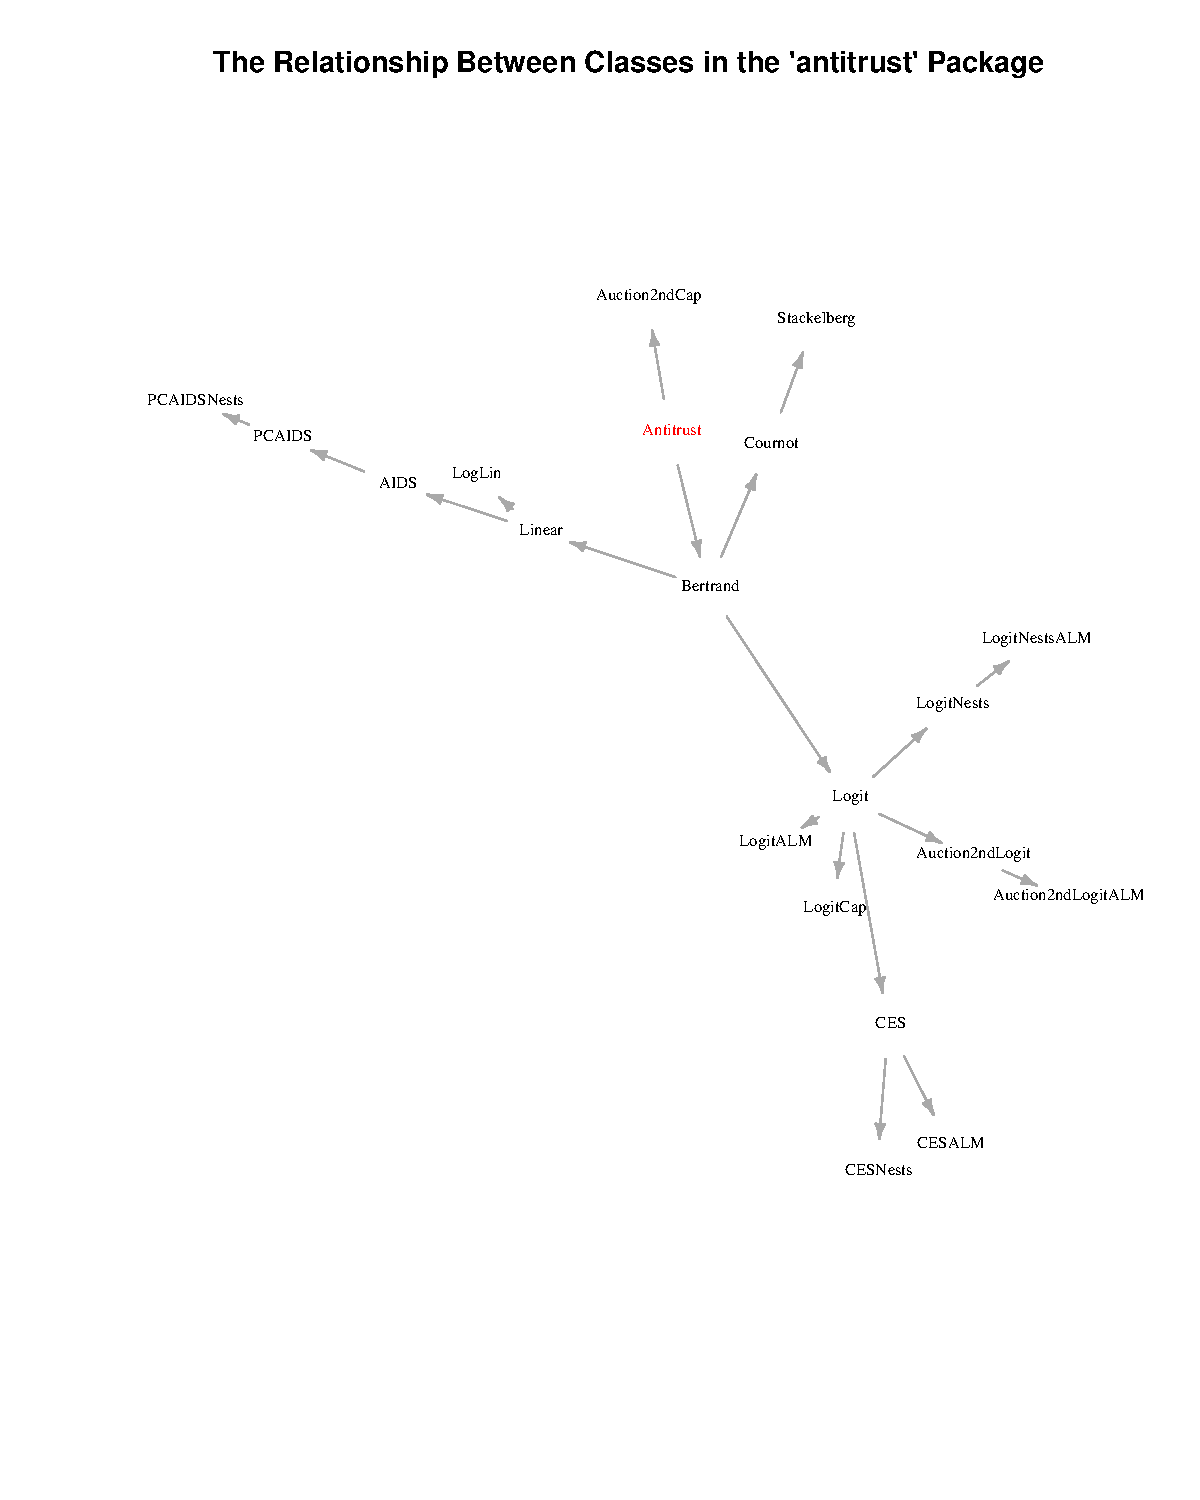
\includegraphics{ClassDiagram.pdf}
\label{fig:S4Classes}
\end{figure}

\bibliography{antitrustbib}
\bibliographystyle{plainnat}

\printindex{}

\end{document}




